\section{Experiments}\label{sec:experiments}
\subsection{Data}\label{subsec:data}

% Data: Describe the dataset(s) you are using (provide references). Being precise about the exact form of the input and output can be very useful for readers attempting to understand your work, especially if you’ve defined your own task. If there are legal or ethical considerations to the data used, discuss it here.

We use a mixture of DPO preference data and MCQA-style SFT datasets.

\textbf{EPFL Preference Data.} This dataset is a collection of 26,738
student-generated answer pairs where one answer is preferred over the other. 
The questions comprise 1,522 unique questions from 24 different courses at
EPFL. Each pair of answers was generated by prompting GPT-3.5 and annotated
using various ranking criteria and an overall ranking by students from the
CS-552 course. Before any further processing, we perform an 80-20
train-validation split.

\textbf{ARC.} The ARC dataset~\cite{arc} consists of 7,787 grade-school
level, multiple-choice science questions released by the Allen Institute for
Artificial Intelligence (AI2). 

\textbf{SciQ.} The SciQ dataset~\cite{sciq} contains 13,679
crowdsourced science exam questions from natural sciences, like physics,
chemistry and biology. Each question is in multiple-choice format and a paragraph of supporting
evidence for the correct answer is available.

\textbf{OpenBookQA.} The OpenBookQA dataset~\cite{openbookqa} is a collection of
5,957 multiple-choice science questions. The dataset is designed to test the
model's ability to answer questions that require reasoning and understanding of
the natural world.

\textbf{MMLU.} The Massive Multitask Language Understanding (MMLU)
benchmark~\cite{mmlu} is a large, diverse collection of multiple-choice
questions from various domains. In this work, we use the MMLU-STEM subset,
consisting of 19 of the subjects most relevant to STEM and 3,317 questions. 

\textbf{GPQA.} The General Purpose Question Answering (GPQA)
benchmark~\cite{gpqa} is a dataset of 1,192 very challenging
multiple-choice questions, designed and validated by experts in natural
sciences. With human expert baseline scores being only 34\%, it is among the
most challenging benchmarks in the industry.

% Example + Formatting
For each dataset, we provide an example data sample in the Appendix
Section~\ref{subsec:data-examples}. Before using the data for fine-tuning or
evaluation, we preprocess it into a standardised format. To do this, we
parse the question, answer options, and correct answer and format them as shown in Appendix Section~\ref{subsec:data-formatting}. We use the chat template used by our base model, and feed the question text, followed by a lettered list of answer options as the user message, and the correct answer as the assistant message.

% Detail usage of each of these data sources
Depending on the availability of training and validation/test splits, we use
the above datasets for fine-tuning and evaluation, or only evaluation. This is detailed in Sections ~\ref{subsec:evaluation} and~\ref{subsec:experimental-details}. All datasets are publicly available on HuggingFace, with the exception of the EPFL preference data which was provided to us by the EPFL course staff.


\subsection{Evaluation}
\label{subsec:evaluation}

% Evaluation method: Describe the evaluation metric(s) you use, plus any other details necessary to understand your evaluation. If you’re defining your own metrics, be clear as to what you’re hoping to measure with each evaluation method (whether quantitative or qualitative, automatic or human-defined!), and how it’s defined.

% Evaluation Benchmarks
For DPO alignment, we evaluate using the model's accuracy in assigning a higher probability to the preferred answer.

% Evaluation Methodology/ Metrics
To evaluate models, we use the LMEH framework, which is commonly used in the literature to evaluate language models and also powers the
HuggingFace's OpenLLM Leaderboard. The framework uses the same methodology of
comparative log-likelihood scoring to extract the model's answer to a
multiple-choice question. Then, given a list of model predictions $\hat{y}_1,
\dots, \hat{y}_n$ and the ground truth answers $y_1, \dots, y_n$ for a task, it
computes the accuracy score as, where $\mathbb{I}(\cdot)$ is the indicator function. Additionally, it computes
the standard error (SE) in the accuracy score which gives an estimate of the uncertainty in the accuracy score given the number
of questions in the benchmark task. We use only zero-shot evaluation for all
benchmarks, as this is how the model would be used if it were chatbot.

\subsection{Baselines}\label{subsec:baselines}
% Baselines: You should also describe your baseline(s).

We first verify that the Phi-3-Mini model is the best performing model on the MCQA benchmarks defined in Section \ref{subsec:data}. We compare against the following two models:

\textbf{OpenELM.} The OpenELM model~\cite{openelm} is a family of small, efficient language models released by Apple in April 2024. We use the largest available, instruction-tuned model, OpenELM-3B-Instruct, for our experiments.

\textbf{Llama 3.} Finally, we consider the models from the popular LLama 3 family~\cite{llama}. In particular, we use LLama-8B-Instruct model, the smallest model in the most recent release of model family by Meta in April 2024.

For all experiments including DPO alignment, MCQA fine-tuning, and quantisation, we use the Phi-3-Mini model as the baseline.

\subsection{Experimental Details}
\label{subsec:experimental-details}

% Experimental details: Report how you ran your experiments (e.g. model configurations, learning rate, training time, etc.).

\textbf{DPO alignment}. We follow two steps for DPO alignment. We first run several experiments on 20\% of EPFL data to tune the parameters outlined in Table~\ref{tab:base-training-setup}. We then identify the best performing configurations based on the validation accuracy and run the train on the full EPFL dataset.

\textbf{MCQA finetuning}. We follow the guidelines for fine-tuning Phi-3 from Microsoft's \href{https://github.com/microsoft/Phi-3CookBook}{cookbook}. Table \ref{tab:sft-setup} details the hyperparameters that differ from Hugging Face's defaults. Using these parameters, we train models on the ARC, SciQ and OpenBookQA datasets, and all in combination. We call these models Phi-3-ARC, Phi-3-SciQ, Phi-3-OBQA, and Phi-3-MCQ respectively.

\textbf{Quantisation}. For the quantisation via GPTQ, we use the default hyperparameters provided by the Hugging Face's API, and only experiment with the number of bits used for quantisation (8, 4, 3, 2).

\subsection{Results}
\label{subsec:results}

% Results: Report the quantitative results that you have found so far. Use a table or plot to compare results and compare against baselines. Comment on your quantitative results. Are they what you expected? Why do you think that is? What does that tell you about your approach?

% We report the results in four stages: First, we present the performance of the three baseline to get an understanding of the trade-off between model size and performance, and the difficulty of the benchmarks. Based on these resutls, we choose our base model. Second, we show DPO alignment resutlts. Third, we present the performance of all variants of our fine-tuned model on the MCQA benchmarks, and compare to the Phi-3-Mini base model. Last but not the least, given the most promising fine-tuned model, we then investigate the effect of of quantisation on the model's performance, showing the results of 8-, 4-, 3- and 2-bit quantised models.

\subsubsection{Baseline Results}

\begin{figure}[ht]
    \centering
    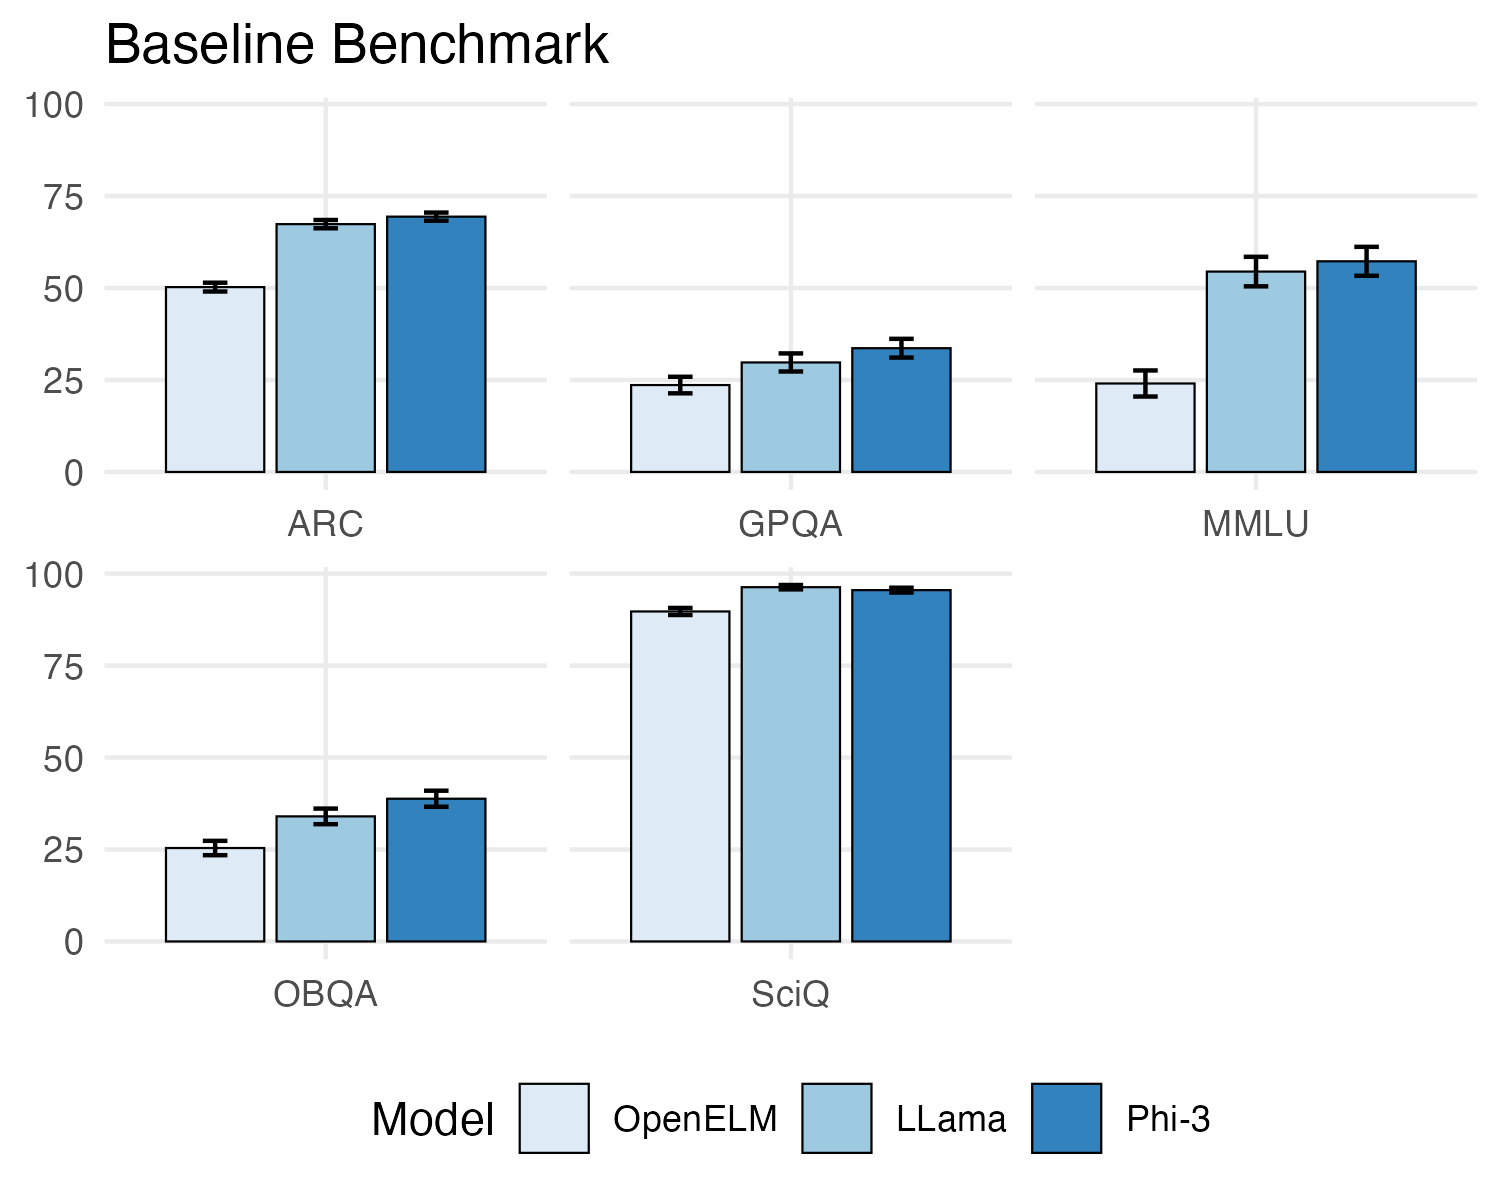
\includegraphics[width=0.45\textwidth]{figures/baseline-benchmark.png}
    \caption{\textbf{Baseline Benchmark Results.} Mean accuracy on all task groups for the three baseline models. Error bars represent the standard error of the accuracy score.}
    \label{fig:baseline-benchmark}
\end{figure}

Figure~\ref{fig:baseline-benchmark} visualises the mean accuracy on all task
groups for the three baseline models (exact numbers are provided in
Appendix Table~\ref{tab:baseline-benchmark}). We observe that OpenELM-3B-Instruct
is worse than the other two models on all benchmarks. While Phi-3 and
LLama-3 perform similarly on most benchmarks, Phi-3 slightly
outperforms LLama-3 on most benchmarks. This is surprising as
Phi-3 is half the size of LLama-3, and similarly
sized as OpenELM-3B. This suggests that Phi-3 is the most performant model for its size among the base models
we consider and provides a strong baseline for our
experiments. However, this also means that it will be more challenging to
improve the model further by fine-tuning.

Moreover, we observe that the benchmarks vary in difficulty. GPQA and OBQA are the most challenging benchmarks with Phi-3 achieving 33.6\% and 38.8\% accuracy respectively. MMLU and ARC are less challenging, with Phi-3 scoring accuracy of 57.3\% and 69.4\%. SciQ is the easiest benchmark, with Phi-3-Mini achieving 95.5\% accuracy.

\subsubsection{DPO Alignment Results}

\begin{table}[ht]
    \small
    \centering
    \caption{Training Configuration and Results for DPO finetuning. On the left, we highlight in bold the hyper-parameters being tuned (LabSm = Label Smoothing).}
    \begin{tabular}{ccccc|c}
        \toprule
        \multicolumn{5}{c}{\textbf{Configuration}} & \textbf{Results} \\
         LR & Rank & Loss & Beta & LabSm & Acc (\%) $\downarrow$\\
        \midrule
        4e-5 & 32 & \textbf{IPO} & \textbf{0.1} & 0.1 & 67.01\% \\
        \textbf{2e-5} & \textbf{16} & \textbf{IPO} & \textbf{0.1} & \textbf{0.0} & 66.61\% \\
        4e-5 & 32 & DPO & \textbf{0.05} & 0.1 & 65.97\% \\
        \textbf{2e-5} & \textbf{16} & DPO & 0.4 & 0.1 & 64.76\% \\
        4e-5 & 32 & DPO & 0.4 & \textbf{0.0} & 63.89\% \\
        4e-5 & 32 & DPO & 0.4 & 0.1 & 63.27\% \\
        \bottomrule
    \end{tabular}
    \label{tab:dpo-results}
\end{table}

Table \ref{tab:dpo-results} presents the validation accuracy of the DPO alignment experiments. The configuration employing the IPO loss demonstrated the highest performance, aligning with expectations given IPO loss's design to enhance model generalisation. Furthermore, through further hyperparameter tuning, we achieved a nearly 4\% increase in accuracy compared to the baseline model. However, combining the best performing configurations from the experiments resulted in only the second best performing model suggesting a strong interdependence among the hyperparameters.


\subsubsection{Fine-Tuning Results}
\begin{figure*}
    \centering
    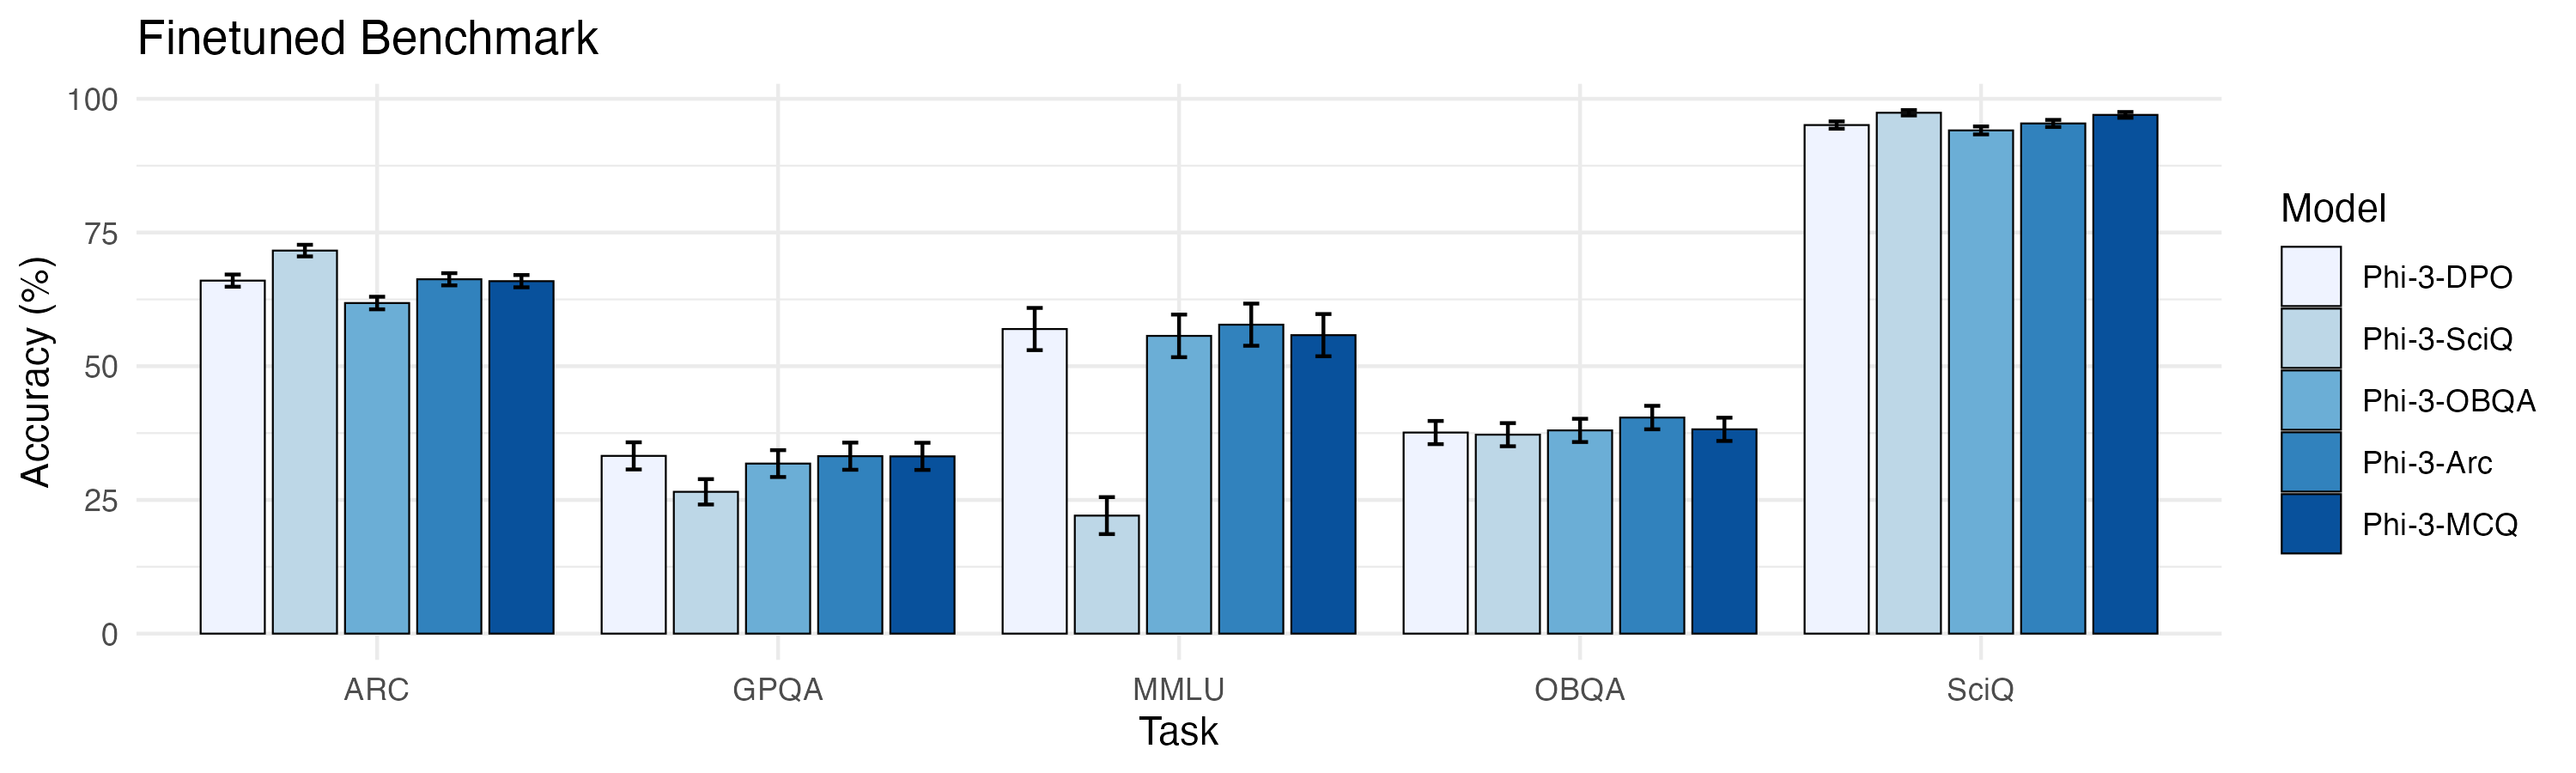
\includegraphics[width=\textwidth]{figures/finetuned-benchmark.png}
    \caption{\textbf{Finetuned Benchmark Results.} Mean accuracy on all task groups for the all fine-tuned models and Phi-3. Error bars represent the standard error of the accuracy score.}
    \label{fig:finetuned-benchmark}
\end{figure*}

Figure~\ref{fig:finetuned-benchmark} shows the mean accuracy on all benchmarks
for all fine-tuned variants, against the Phi-3 baseline, with full results in the Appendix~\ref{tab:finetune-benchmark}. 

% DPO-finetune
Despite the model's increased performance in accuracy in retrieving the preferred answer, performance on
scientific MCQA benchmarks does not improve. We hypothesise that the DPO examples are not similar enough to
MCQA examples in terms of style and content for the training to be transferrable. Aligning
the model towards long answers with explanation does not necessarily benefit the
retrieval of the correct answer from the log-probabilities assigned to the short
answer option continutations used in our evaluation setup. For this reason, we
choose to focus on fine-tuning the base model on highly curated MCQA datasets
that are specifically formatted for the task.


% MCQ-finetune
Fine-tuning on the MCQA datasets does not lead to significant
improvements across the benchmark tasks either. For variants fine-tuned on OBQA, ARC
and a combination of all MCQA datasets, we observe negligible changes in the mean
accuracy that often fall within the standard error of the Phi-3-Mini baseline.
Notably, fine-tuning on SciQ leads to a significant drop in performance on the
MMLU dataset, as well as the GPQA dataset, which suggests a big discrepancy in these datasets.


% Best model
As our final model we choose Phi-3-ARC. It
performs similarly to the strong Phi-3-Mini base model, with a slight increase in
performance on the MMLU and OBQA benchmarks, from 57.3\% to 57.8\% and 38.8\% to
40.4\% respectively.

\subsubsection{Quantisation}

\begin{figure}[ht]
    \centering
    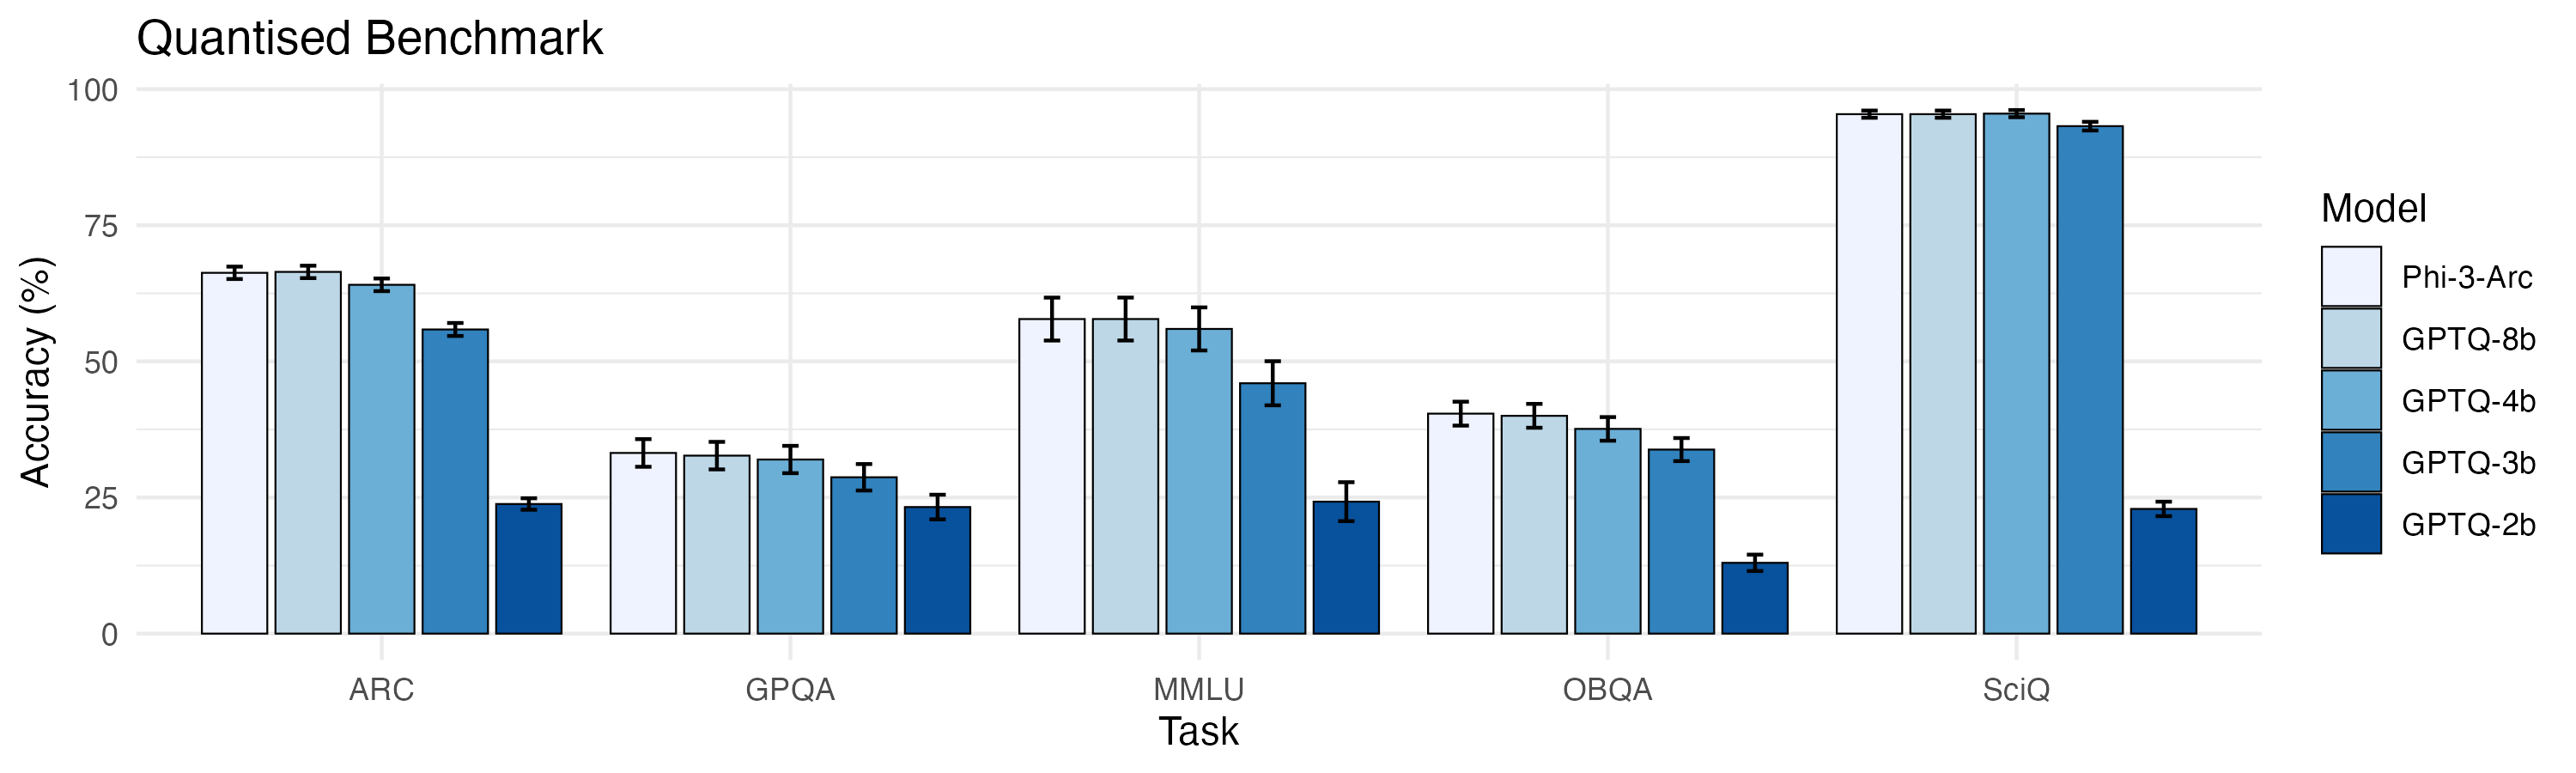
\includegraphics[width=0.45\textwidth]{figures/quantised-benchmark.png}
    \caption{\textbf{Quantised Benchmark Results.} The Figure shows the accuracy of the quantised models and its unquantised counterpart on the benchmarks. The error bars represent the standard error of the accuracy score.}
    \label{fig:quantised-benchmark}
\end{figure}

We quantise the Phi-3-ARC model and show
the results of 8-, 4-, 3- and 2-bit variants in
Figure~\ref{fig:quantised-benchmark}.

% Quantisation results
We find that quantising using GPTQ is an effective approach to reducing the
memory footprint of the model while maintaining the impressive MCQA performance. The 8-bit, and 4-bit quantised models perform similarly to the unquantised model across all benchmarks. However, when further quantising to 3-bit precision, we observe a decrease in the performance, with the mean accuracy dropping to 57.3\% on the MMLU benchmark. Finally, 2-bit quantisation is not feasible for our model, as we find that it performs no better than a random baseline.

% Best model
We conclude that the 4-bit quantised model provides the best trade-off between
performance and efficiency, and choose this model as our final quantised model
for submission.

